\clearpage

\lehead[]{\normalfont\sffamily\hspace*{-2.00cm}\textcolor{white}{\colorbox{lightblue}{\parbox[c][0.70cm][b]{1.60cm}{
\makebox[1.60cm][r]{\thechapter}\\ \makebox[1.60cm][r]{ÜBUNG}}}}\hspace{0.17cm}\textcolor{lightblue}{\chaptertitle}}
\rohead[]{\textcolor{lightblue}{\chaptertitle}\normalfont\sffamily\hspace*{0.17cm}\textcolor{white}{\colorbox{lightblue}{\parbox[c][0.70cm][b]{1.60cm}{\thechapter\\
ÜBUNG}}}\hspace{-2.00cm}}
%\chead[]{}
\rehead[]{\textcolor{lightblue}{AvHG, Inf, My}}
\lohead[]{\textcolor{lightblue}{AvHG, Inf, My}}

\section{Komplexe Dialogelemente -- Übungen}

\subsection{Aufgabe 1: Einkaufsliste}

Programmiere einen elektronischen Einkaufszettel.

\begin{center}
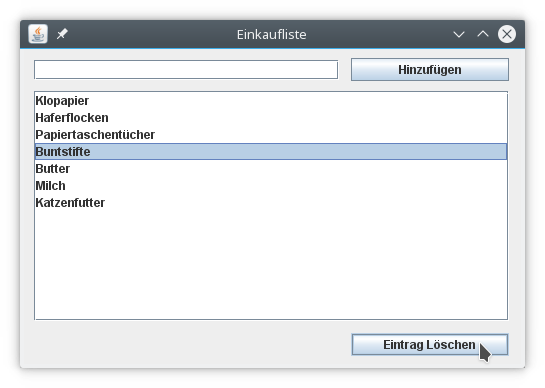
\includegraphics[width=0.8\textwidth]{./inf/SEKII/24_Java_GUI-Komponenten/Einkaufsliste.png}
\end{center}

Text, der in dem Textfeld eingegeben wurde, soll durch betätigen des Buttons zum
Hinzufügen in das Datenmodell der \myClass{JList}-Komponente übernommen werden.
Übrigens kannst du auch dem Textfeld einen \myClass{ActionListener} spendieren
und dort ebenfalls die Methode zum Hinzufügen zur Liste aufrufen. Dann reicht es
im Textfeld nach Eingabe eines neuen Eintrags die Eingabetaste zu drücken und
schon landet der Eintrag genauso in der Einkaufsliste, als wenn der Button
gedrückt worden wäre.

Außerdem soll es möglich sein, den jeweils ausgewählten Listeneintrag aus dem
Datenmodell der \myClass{JList}-Komponente zu löschen. Geschickter Weise sollte
die \myClass{JList}-Komponente so im WindwoBuilder eingestellt werden, dass man
jeweils nur einen Listeneintrag auswählen kann (\myCmd{selectionMode}
$\rightarrow$ \myCmd{SINGLE\_SELECTION}).
